%!TEX encoding = IsoLatin

%
% Annexe "Équations de la caméra custom"
%

\chapter{Équations pour le capteur d'image OV5640}
\label{annexe:equation_camera_custom}

Dans cette annexe, toutes les équations nécessaires à la compréhension des données de la section \ref{subsubsection:camera_custom} seront fournies.

Les spécifications du fabriquants nécessaires aux calculs sont indiqués au tableau \ref{t:specs_camera_custom}.

\begin{table}[!htb]
\footnotesize
\centering
    \begin{tabular}{|c|c|}
    \hline
    Specs & Valeur\\
    \hline\hline
    Taille du pixel & 1.4$\mu$m\\
    Hauteur du senseur ($H$) & 2738.4 $\mu$m\\
    Largeur du senseur ($W$) & 3673.6 $\mu$m\\
    Focale & 3.2mm\\
    F-number & 2.8\\
    \hline
    \end{tabular}
\caption{Spécification du fabriquant pour le capteur OV5640 \cite{OV5640}}
\label{t:specs_camera_custom}
\end{table}

Pour l'exemple de calcul, les données suivantes du tableau \ref{t:ex_calcul_camera_custom} seront considérées. Celles-ci sont possible selon les données fournies par le fabriquant. Le diamètre de la lentille est déterminé à partir du F-number $N=f/D$ et le cercle de confusion est calculé comme $c=1.5 t_\text{px}$
\begin{table}[!htb]
\footnotesize
\centering
    \begin{tabular}{|c|c|}
    \hline
    Specs & Valeur\\
    \hline\hline
    Focale ($f$) & 3.2mm\\
    F-number ($N$) & f/2.8\\
    Diamètre de la lentille ($D$) & 1.143mm\\
    Distance du focus ($s$) & 1.0m\\
    Distance lentille-capteur ($d$) & 3.2mm\\
    Cercle de confusion ($c$) &  2.1 $\mu$m\\
    \hline
    \end{tabular}
\caption{Valeurs pour un exemple de calcul}
\label{t:ex_calcul_camera_custom}
\end{table}

Les équations \ref{eq:distance_hyperfocale} à \ref{eq:champ_lointain} sont les équations d'imagerie \cite{Photographic_optics}. La distance hyperfocale $H$ est une nécessaire pour calculer la profondeur de champ:
\begin{equation}
    H = \frac{f^2}{Nc} - f
    \label{eq:distance_hyperfocale}
\end{equation}

Le champ proche $D_n$ est la limite inférieure à laquelle le système peut imager:
\begin{equation}
    D_n = \frac{s(H-s)}{H+s-2f}
    \label{eq:champ_proche}
\end{equation}

Le champ lointain $D_f$ est la limite supérieure à laquelle le système peut imager:
\begin{equation}
    D_n = \frac{s(H-s)}{H-s}
    \label{eq:champ_lointain}
\end{equation}

\begin{figure}[!htb]
    \centering
    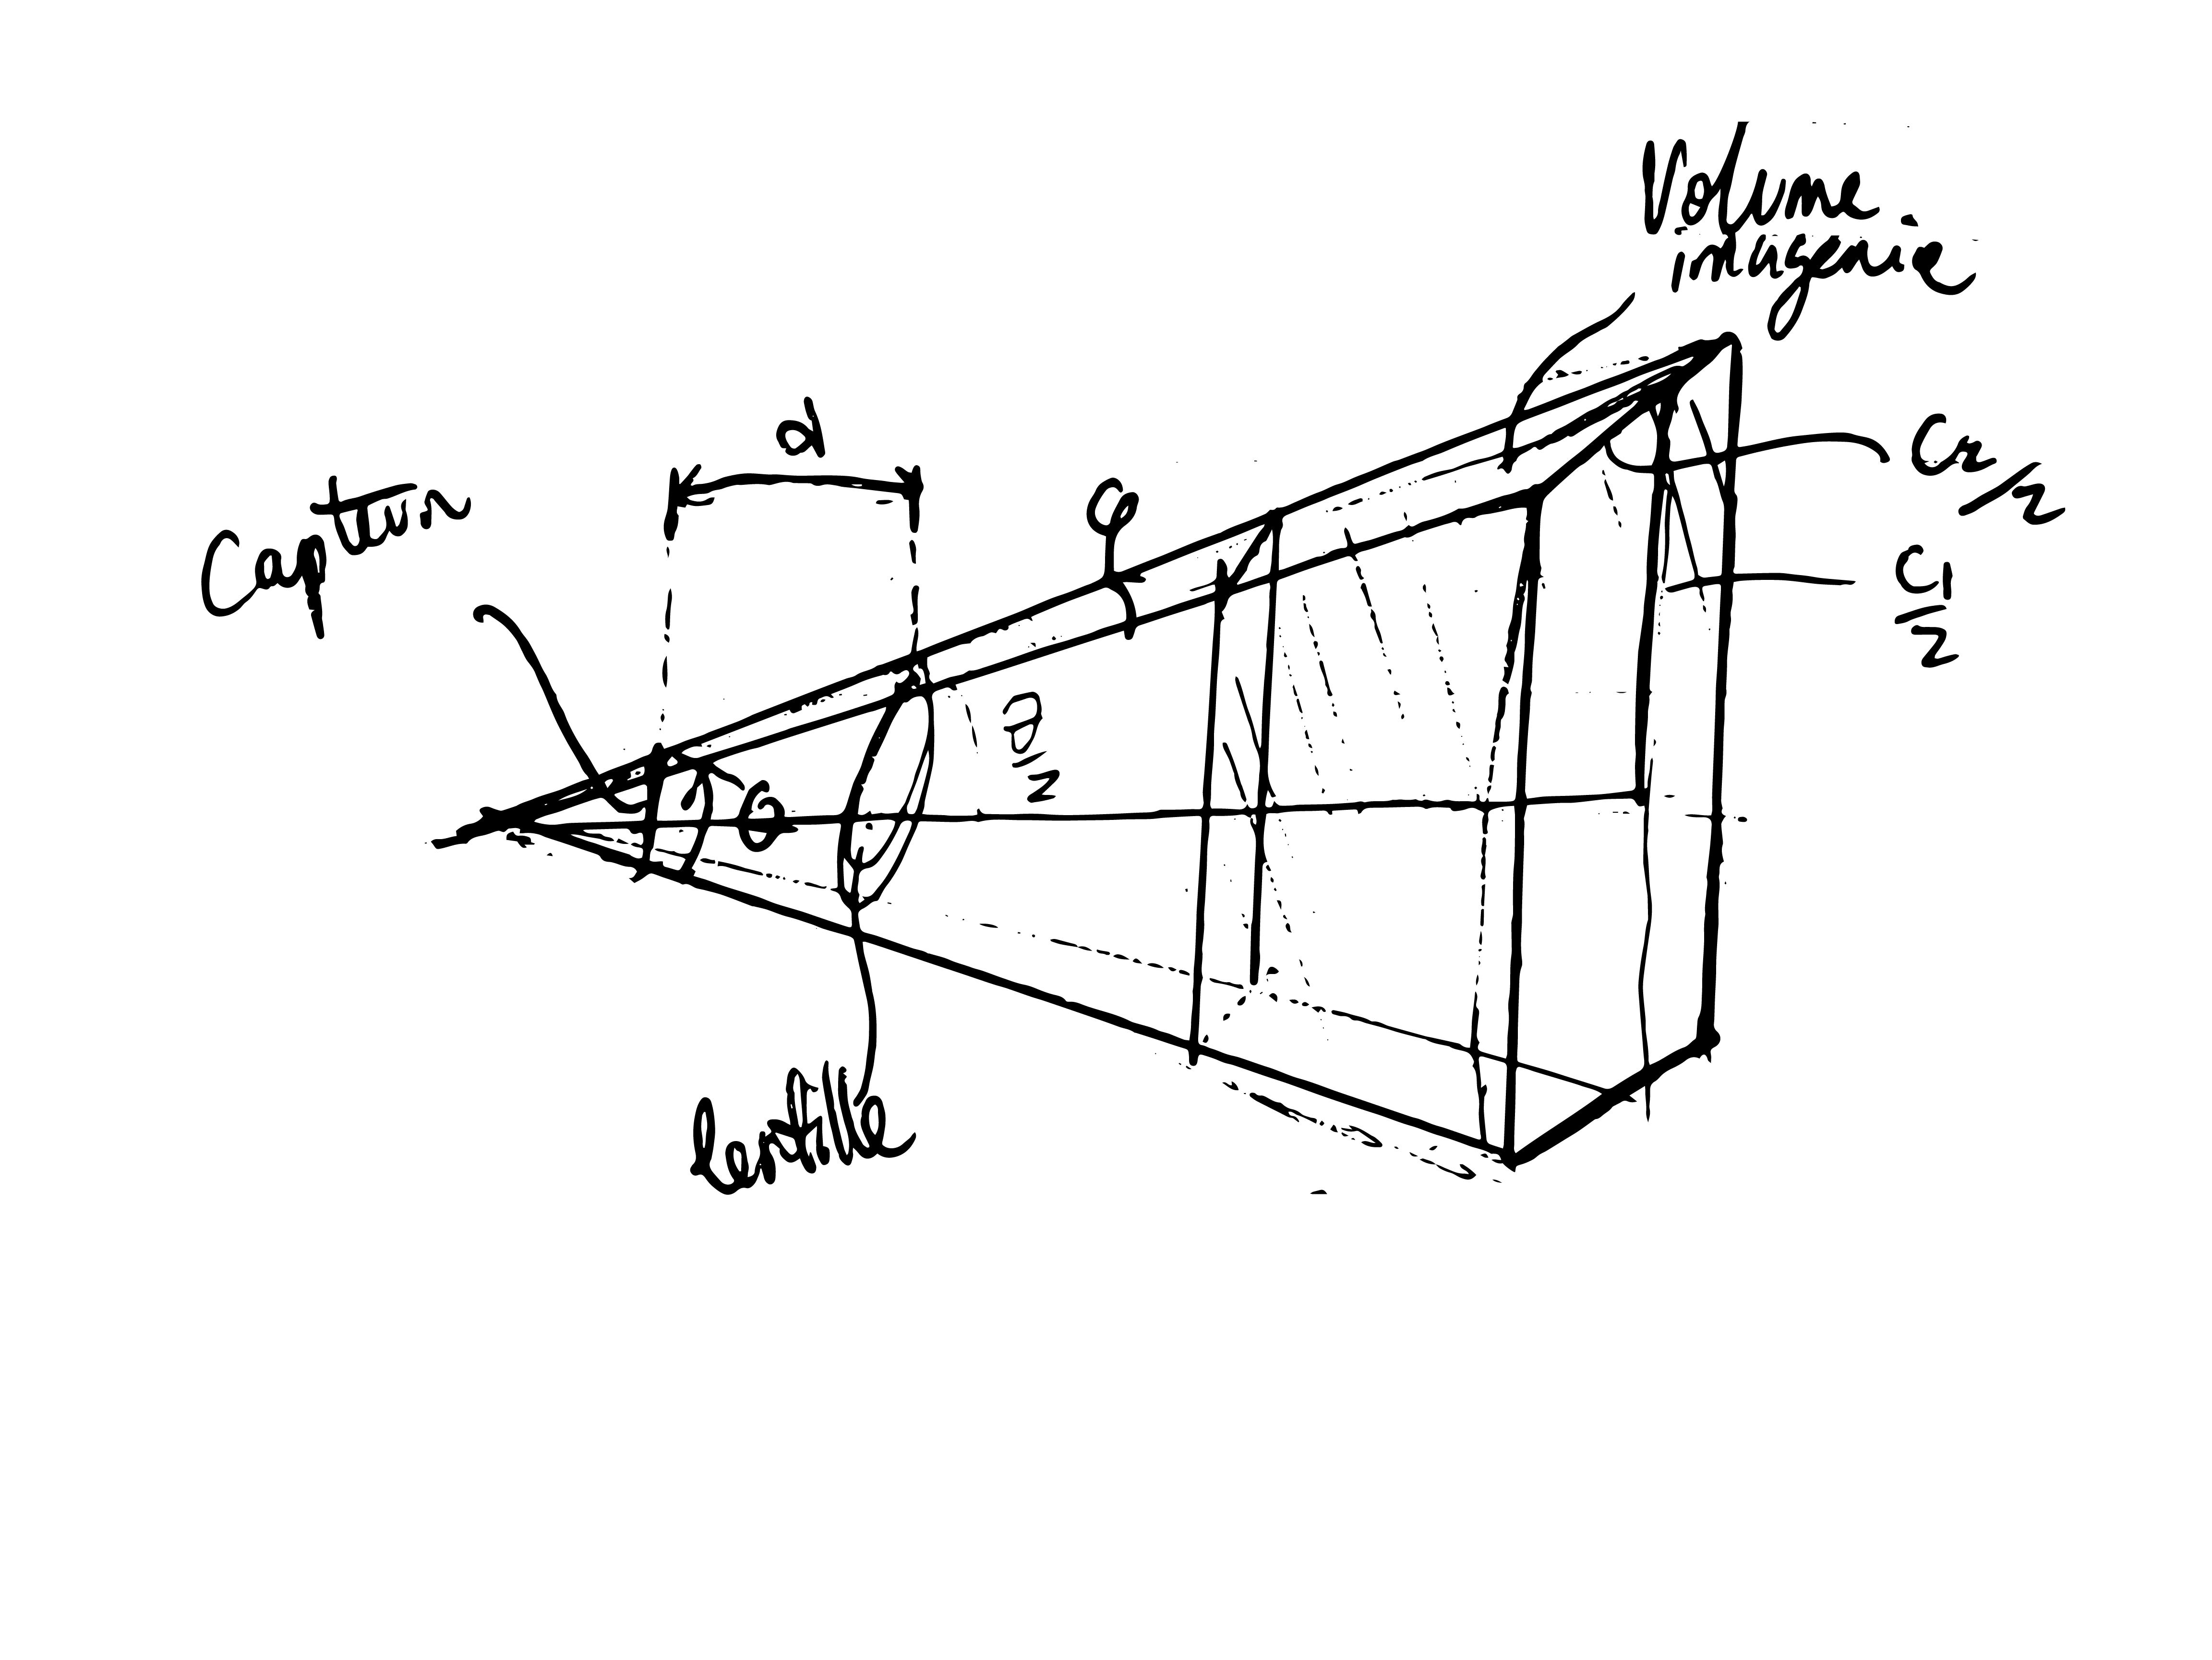
\includegraphics[width=0.5\linewidth]{fig/camera_custom_geometrie_vect.png}    \caption{Géométrie du volume d'imagerie}
    \label{fig:volume_imagerie}
\end{figure}


Le volume d'imagerie est une pyramide tronquée. Le développement de son équation nécessite donc les équations d'imagerie et les équations de la géométrie du système. Les équations \ref{eq:base_lointaine} à \ref{eq:angles} définissent la géométrie du système à la figure \ref{fig:volume_imagerie}. L'aire de la base la plus lointaine $Ab_f$ est définie un rectangle tel que
\begin{align}
    Ab_f &= c_{1f} \cdot c_{2f}\\
    c_{1f} &\equiv 2D_f \tan{\frac{\theta}{2}}\\
    c_{2f} &\equiv 2D_f \tan{\frac{\phi}{2}}\\
    Ab_f &= (2 D_f)^2 \tan{\frac{\theta}{2}} \tan{\frac{\phi}{2}}
    \label{eq:base_lointaine}
\end{align}

L'aire de la base la plus proche $Ab_n$ est définie un rectangle tel que
\begin{align}
    Ab_n &= c_{1n} \cdot c_{2n}\\
    c_{1n} &\equiv 2D_n \tan{\frac{\theta}{2}}\\
    c_{2n} &\equiv 2D_n \tan{\frac{\phi}{2}}\\
    Ab_n &= (2 D_n)^2 \tan{\frac{\theta}{2}} \tan{\frac{\phi}{2}}
    \label{eq:base_proche}
\end{align}


\begin{figure}[!htb]
    \centering
    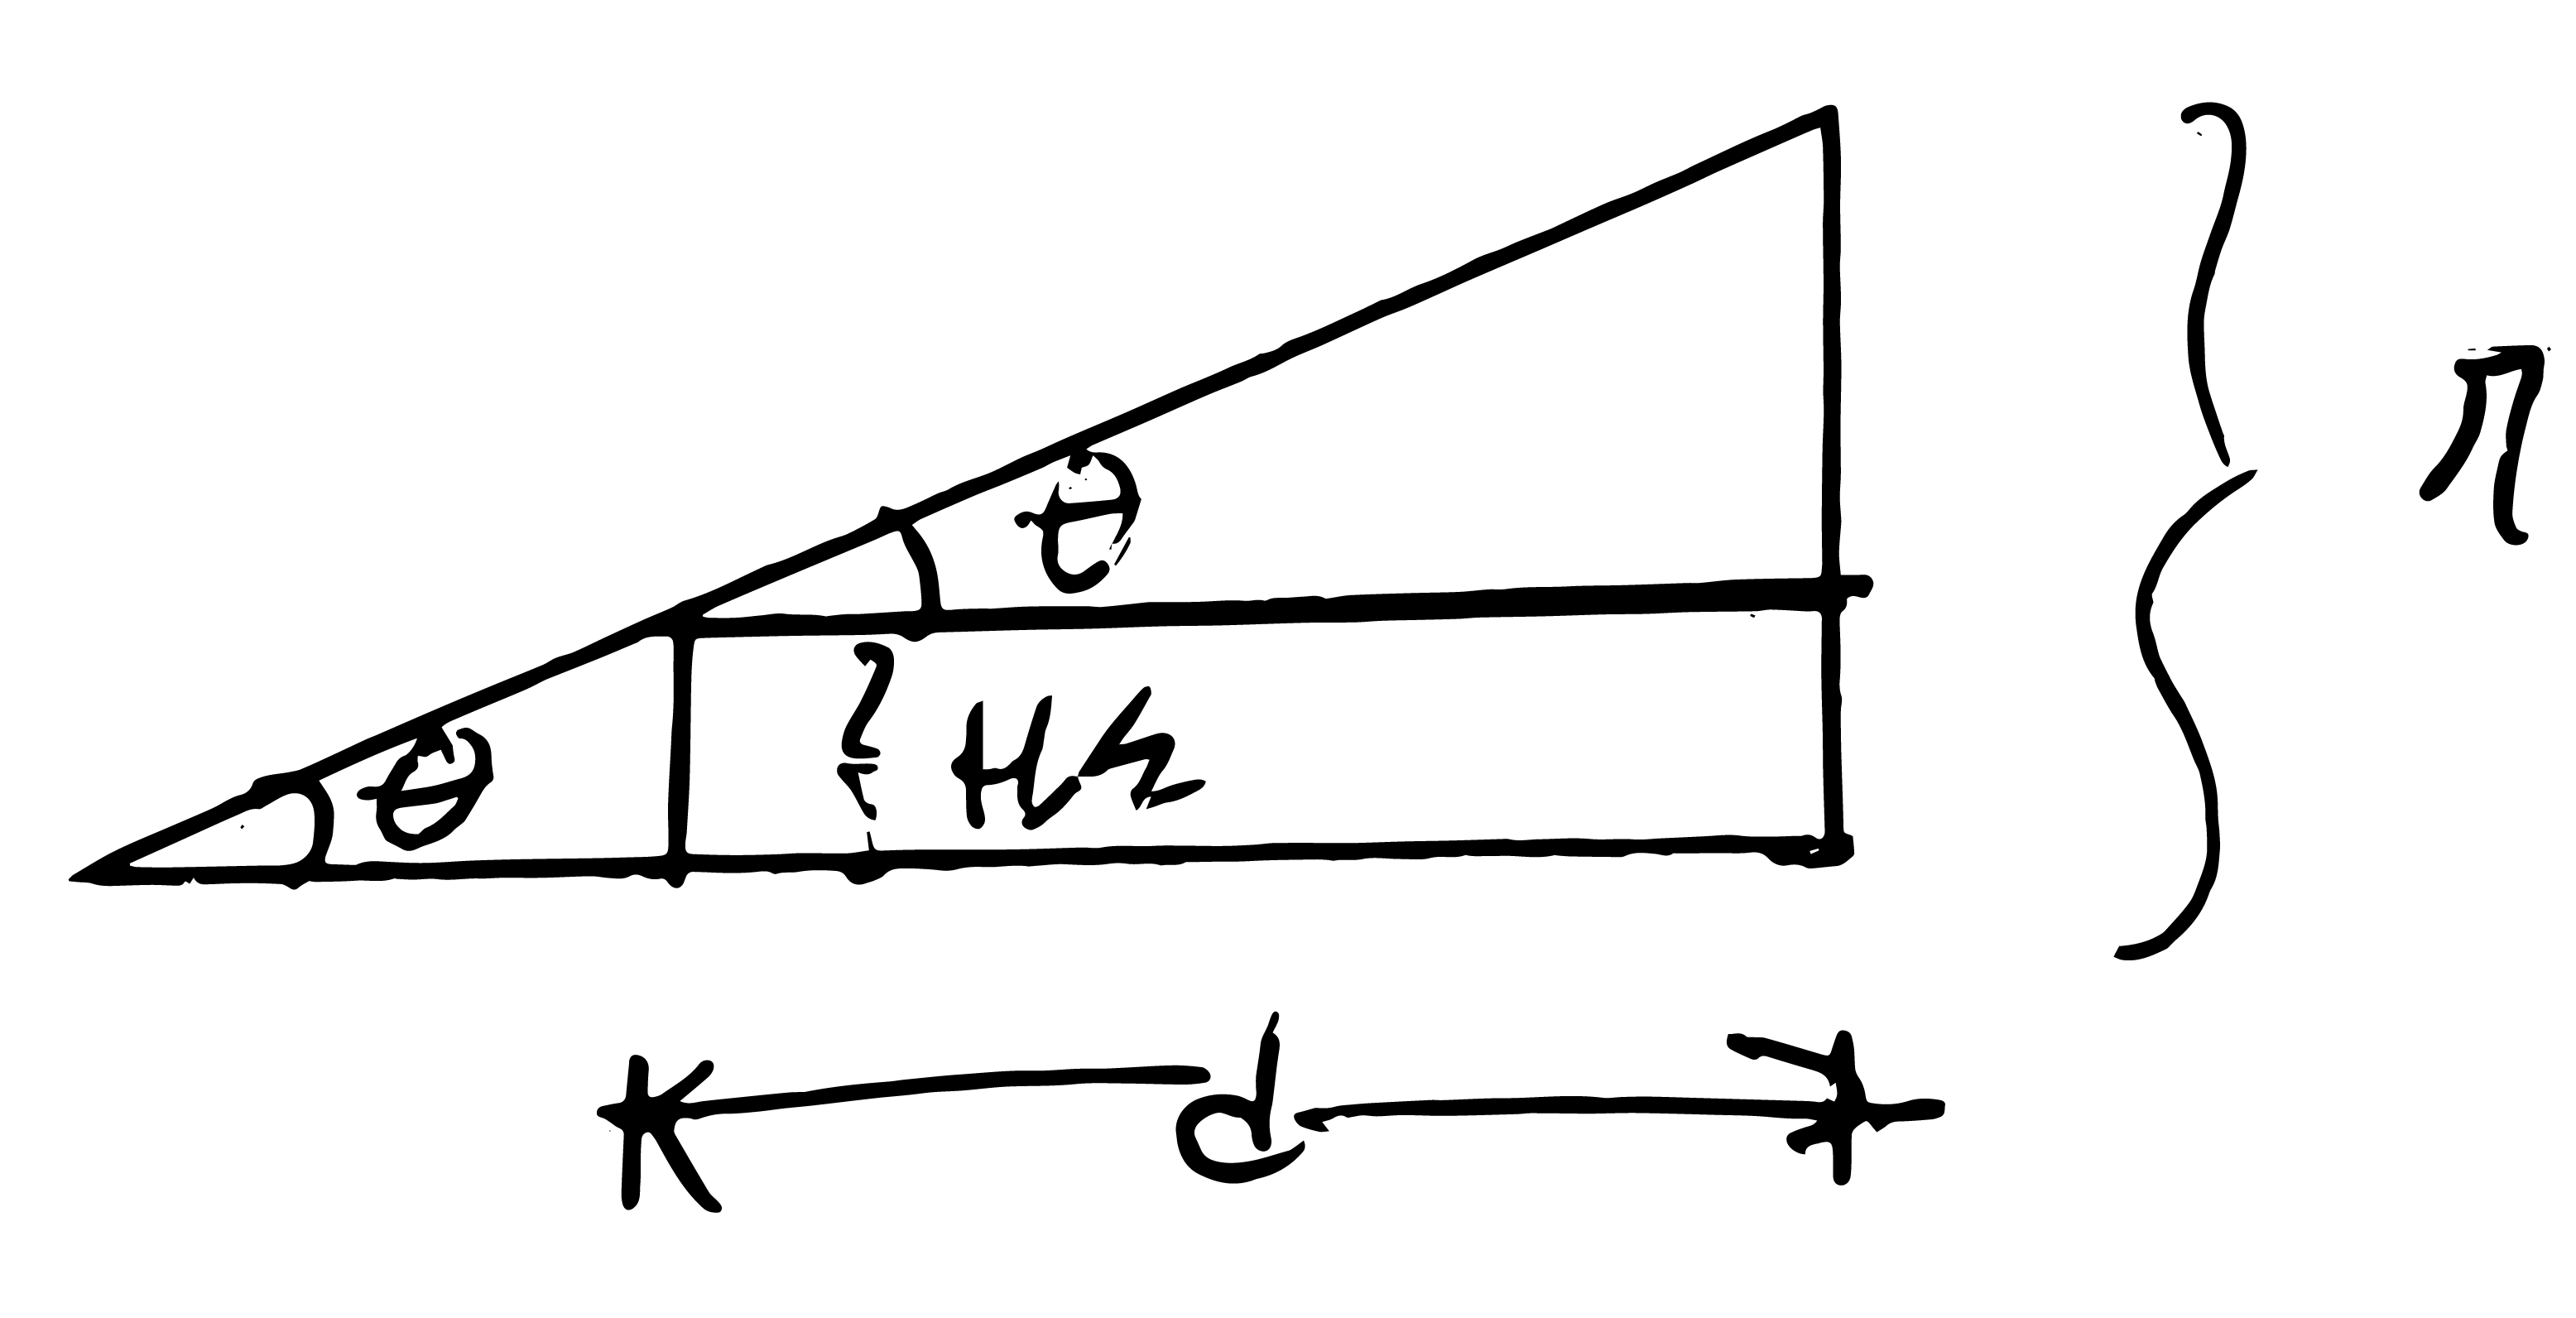
\includegraphics[width=0.5\linewidth]{fig/camera_custom_angle_vect.png}
    \caption{Géométrie du système lentille-capteur}
    \label{fig:lentille_capteur}
\end{figure}

À l'aide du système lentille-capteur, il est possible de déterminer une relation pour les angles $\phi$ et $\theta$ en supposant que l'ouverture du champ est limitée par le diamètre de la lentille.
\begin{align}
    \tan{\frac{\theta}{2}} &= \frac{r-H/2}{d}\\
    \tan{\frac{\theta}{2}} &= \frac{D-H}{2d}\\
    \tan{\frac{\phi}{2}} &= \frac{r-W/2}{d}\\
    \tan{\frac{\theta}{2}} &= \frac{D-W}{2d}
    \label{eq:angles}
\end{align}

En combinant toutes ces équations, il est possible d'arriver à la relation suivante:
\begin{align}
    V &= \frac{Ab_f D_f}{3} - \frac{Ab_n D_n}{3}\\ 
    V &= \frac{4 \tan{\frac{\theta}{2}}  \tan{\frac{\phi}{2}}}{3} \left( D_f^3 - D_n^3\right)\\
    V &= \frac{4}{3} \left(\frac{D-H}{2d} \right) \left(\frac{D-W}{2d} \right) \left( D_f^3 - D_n^3\right)
    \label{eq:volume_imagerie}
\end{align}

On obtient alors les résultats montrés au tableau \ref{t:resultat_calcul_camera_custom}.
\begin{table}[!htb]
\footnotesize
\centering
    \begin{tabular}{|c|c|}
    \hline
    Specs & Valeur\\
    \hline\hline
    Hyperfocale & 1.738m\\
    Limite de champ proche $D_n$ & 0.635m\\
    Limite de champ lointain $D_f$ & 2.350m\\
    Angle d'ouverture $\theta$ & -27.997°\\
    Angle d'élévation $\phi$ & -43.151°\\
    Volume d'imagerie & 1.672m$^3$\\
    \hline
    \end{tabular}
\caption{Résultat de l'exemple de calcul}
\label{t:resultat_calcul_camera_custom}
\end{table}


\chapter{Équations pour le boitier}
\label{annexe:equation_boitier}

La pression hydrostatique est définie à l'équation \ref{eq:profondeur}. La profondeur est $h$ et $p_0$ est la pression atmosphérique.

\begin{equation}
    p = p_0 +\gamma_\text{eau} h
    \label{eq:profondeur}
\end{equation}

Ainsi, la pression à une profondeur de 15.25m est de 250.9kPa.

\begin{align}
    p &= p_0 +\gamma_\text{eau} h\\
    &= 101.3\text{kPa} + 9.807\text{kN/m}^3 \cdot 15.25m\\
    &= 101.3\text{kPa} + 149.6\text{kPa}\\
    p &= 250.9\text{kPa}
\end{align}

Selon le design du boitier à la figure \ref{fig:boitier_camera_custom}, les caractéristiques seraient les suivantes 

\begin{table}[!htb]
\footnotesize
\centering
    \begin{tabular}{|c|c|c|}
    \hline
    Caractéristique & Aluminium & PMMA\\
    \hline\hline
    Surface & 6$\cdot$ 0.04m$^2$ & 0.04m$^2$\\
    Épaisseur & 6mm & 2mm\\
    Masse pour la commande & 4.032kg & 0.095kg\\
    Coût & 2.6\$/kg & 3.70\$/ft$^2$ \\
    \hline
    Coût total & 10.50\$ & 1.59\$ \\
    \hline
    \end{tabular}
\caption{Caractéristiques pour la commande des matériaux du boitier \cite{PMMA_cout} \cite{Aluminium_cout}}
\label{t:commande_boitier}
\end{table}

La masse d'aluminium dans le dispositif est
\begin{align}
    m &= \rho_{Al} V\\
    V &= c^3 - (c-t)^3\\
    V &= (0.2m)^3 - (0.2m - 0.006m)^3\\
    V &= 6.99 \cdot 10^{-4} m^3\\
    m &= 2800 kg/m^3 \cdot 6.99 \cdot 10^{-4}m^3\\
    m &= 1.956 kg
\end{align}

La masse de PMMA dans le dispositif est
\begin{align}
    m &= \rho_{PMMA} V\\
    V &= \pi r^2 t\\
    V &= \pi (0.075m)^2 (0.002m)\\
    V &= 3.53 \cdot 10^{-5} m^3\\
    m &= 1190 kg/m^3 \cdot 3.53 \cdot 10^{-5} m^3\\
    m &= 0.042 kg
\end{align}

Le boitier aurait donc une masse de 2.00kg.
